\begin{figure}[p]
\lstset{frame=single}
\begin{tabular}[t]{@{}c@{ }c@{}}
\begin{minipage}{0.35\textwidth}
\begin{lstlisting}
public class A {
  private int x, y;
  public void f() {
    g();
  };
  public void g() {
    this.y = 0;
  }
}

public class B
          extends A {
  private int z;
  public void g() {
    this.z = 0;
  }
  public void h() {}
}
\end{lstlisting}
\end{minipage}
&
\begin{minipage}{0.64\textwidth}
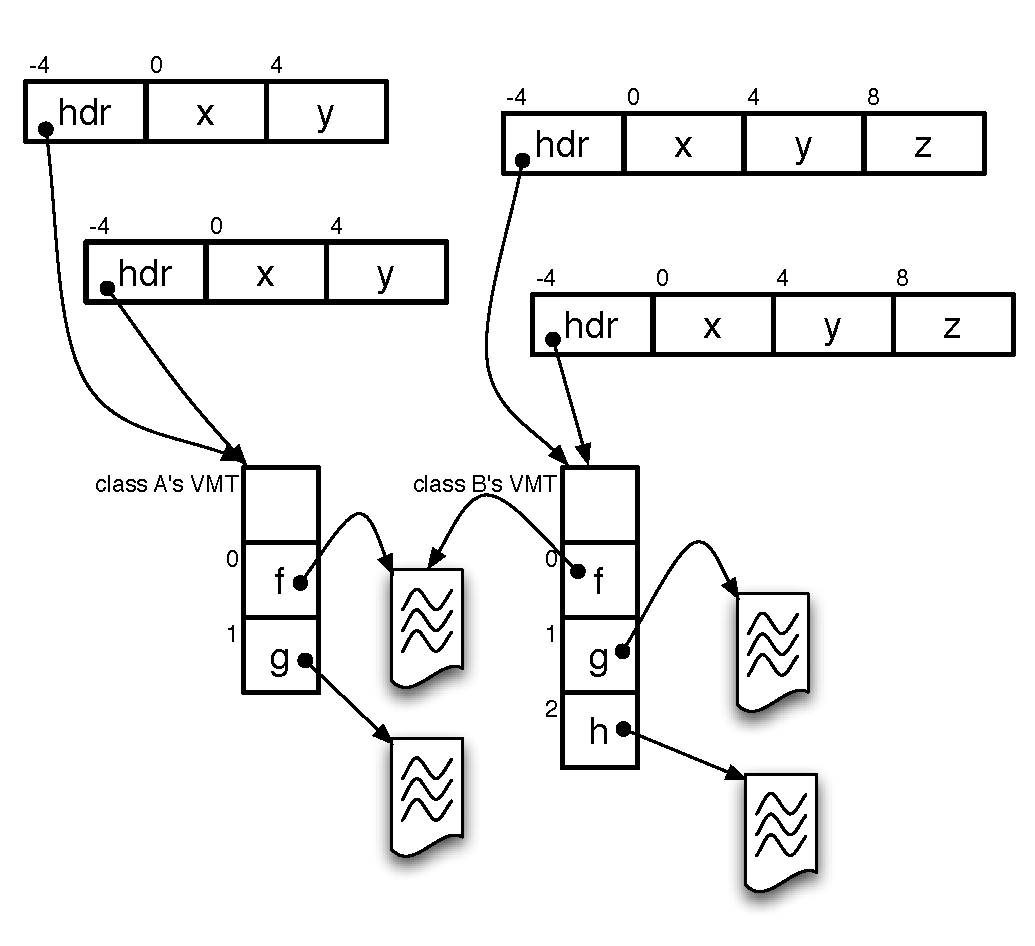
\includegraphics[draft=false,scale=0.5]{100-images/field-method-access-explanation}
\end{minipage} \\
\begin{minipage}{0.28\textwidth}
(a) Java source code
\end{minipage} &
\begin{minipage}{0.44\textwidth}
(b) Objects and VMTs in the heap
\end{minipage} \\[2ex]
\begin{minipage}{0.35\textwidth}
\begin{lstlisting}
aload_0
invokevirtual <A.g>
return
\end{lstlisting}
\vspace{-2ex}
\BC (a) Bytecode for A.f() \EC
\end{minipage} &
\begin{minipage}{0.55\textwidth}
\lstset{moredelim=[il][commentstyle]{>}}
\begin{lstlisting}
>The stack pointer points to "this"
>EDX := this
        MOV     EDX      [ESP]
>The VMT is at offset -4
>ECS := VMT
        MOV     ECX   -4[EDX]
>Send this parameter in EAX
>EAX := this
        MOV     EAX      [ESP]
>Call function g()
>g() is at offset 8 within VMT
        CALL 8[ECX]
\end{lstlisting}
\end{minipage} \\
% \begin{minipage}{0.28\textwidth}
% (c) Bytecode for A.f()
% \end{minipage} &
&
\begin{minipage}{0.38\textwidth}
(d) Machine code for the {\tt invokevirtual} instruction
\end{minipage} \\
\end{tabular}
\hangcaption{Simple example of method and field accesses to illustrate how
inheritance is implemented in Java}
\label{fig:field-method-access-explanation}
\lstset{frame=none}
\end{figure}
